\section{Parallelization}
\label{sec:parallelization}

%The ease with which an algorithm can be parallelized and its performance is important for handling large-scale graphs in emerging applications, where graphs with millions (or more) vertices have become quite common. 

 We demonstrate in this section how our exact algorithm can be parallelized and show performance results
on a shared-memory platform. The heuristic can be parallelized following a similar procedure.

%We here describe the parallelization procedure for both shared and distributed memory architecture. 
As explained in Section \ref{sec:algorithms}, the $i$th iteration of the {\em for} loop in the exact algorithm (Algorithm 1) computes the size of the largest clique that contains the vertex $v_i$. Since our algorithm does not impose any specific order in which vertices have to be processed, these iterations can in principle be performed concurrently. During such a concurrent computation, however, different processes might discover maximum cliques of different sizes---and for the pruning steps to be most effective, the current globally largest maximum clique size needs to be communicated to all processes as soon as it is discovered. In a shared-memory programming model, the global maximum clique size can be stored as a shared variable accessible to all the processing units, and its value can be updated by the relevant processor at any given time. In a distributed-memory setting, more care needs to be exercised to keep the communication cost low. 
%For the distributed case, the effects of pruning could, however, be tolerably compromised in order to enable the parallel computation. This can, for example, be done by using the most recent value of the maximum clique size for pruning, and updating this value by having synchronization steps at regular intervals.

We implemented a shared-memory parallelization based on the procedure described above using OpenMP. Since the global value of the maximum clique is shared by all processing units, we embed the step that updates the maximum clique, i.e. Line \ref{critical} of Algorithm \ref{alg:mClq}, into a {\it critical} section (an OpenMP feature that enforces a lock, thus allowing only one thread at a time to make the update). Further, we use dynamic load scheduling, since different vertices might return different sizes of maximum clique resulting in different work loads.
%, so would work best for our case.

We performed experiments on the same graphs listed in the testbed described in Section \ref{sec:experiments}. For these, we used a Linux workstation 
%running 64-bit version Red Hat Enterprise Linux Server release 6.2 
with six 2.00 GHz Intel Xeon E7540 processors. Each processor has six cores, each with 32 KB of L1 and 256 KB of L2 cache, and each processor shares an 18 MB L3 cache.  
%Implementation was in C++ using OpenMP and compiled with gcc (version 4.4.7) using the -O3 optimization flag.


\begin{figure}
  \centering
    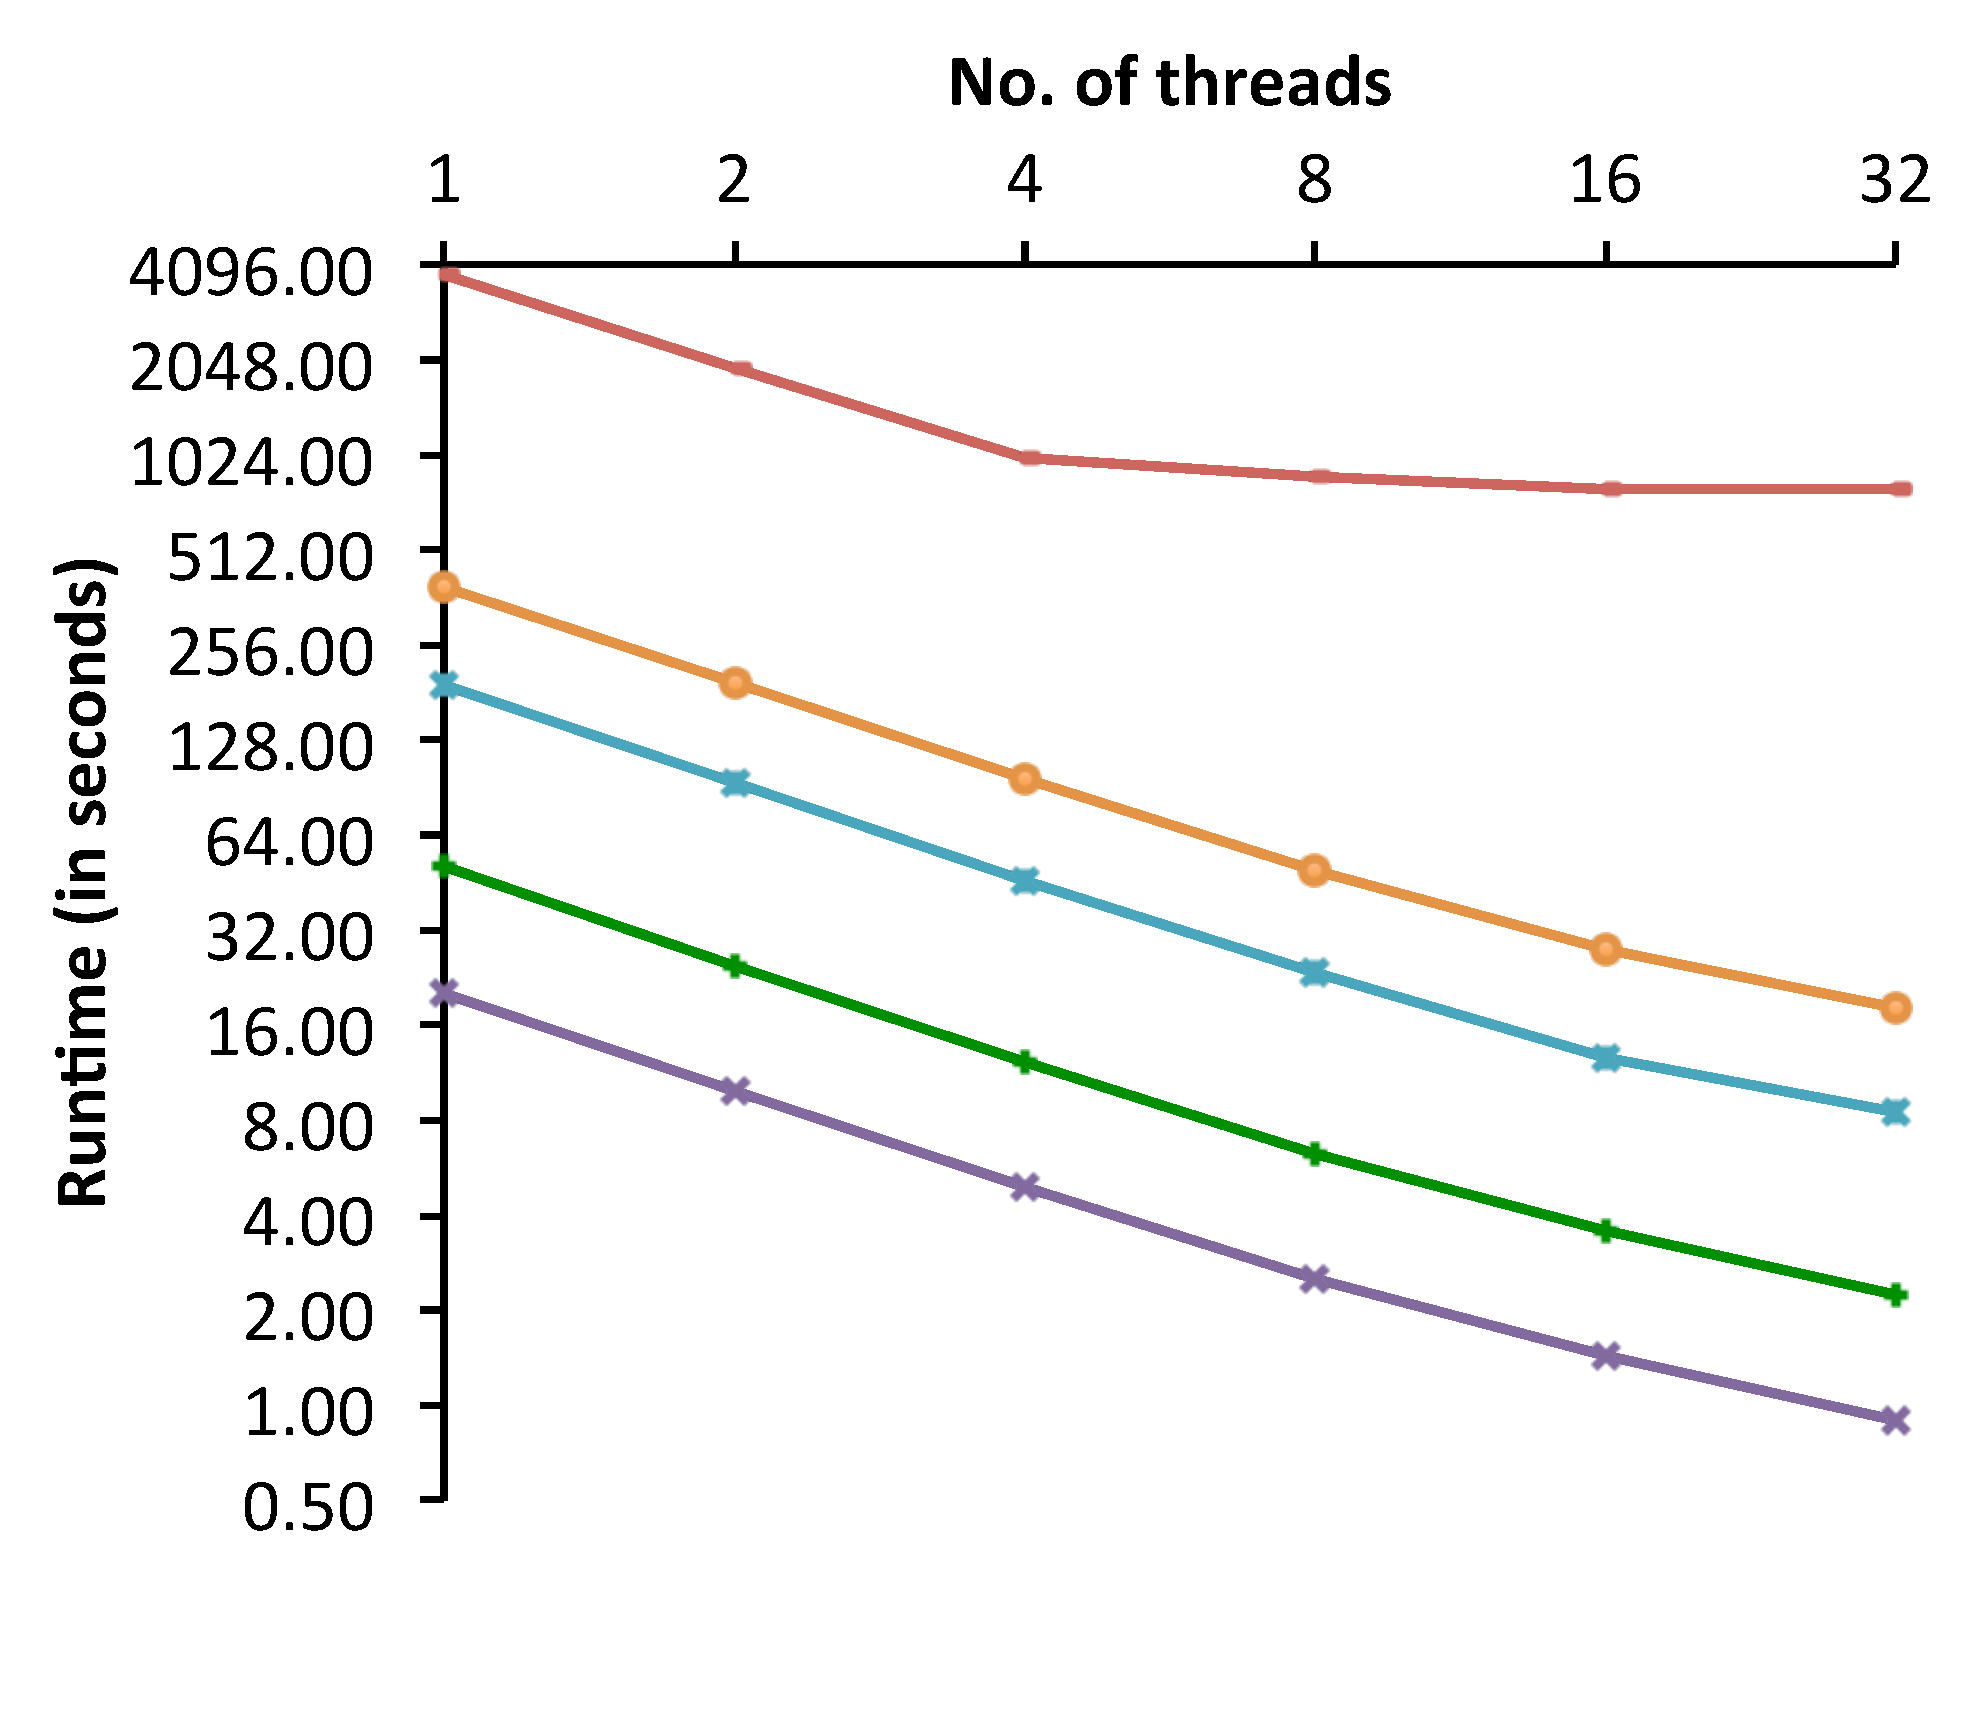
\includegraphics[scale=0.21]{parallel_realworld_timing.pdf}
    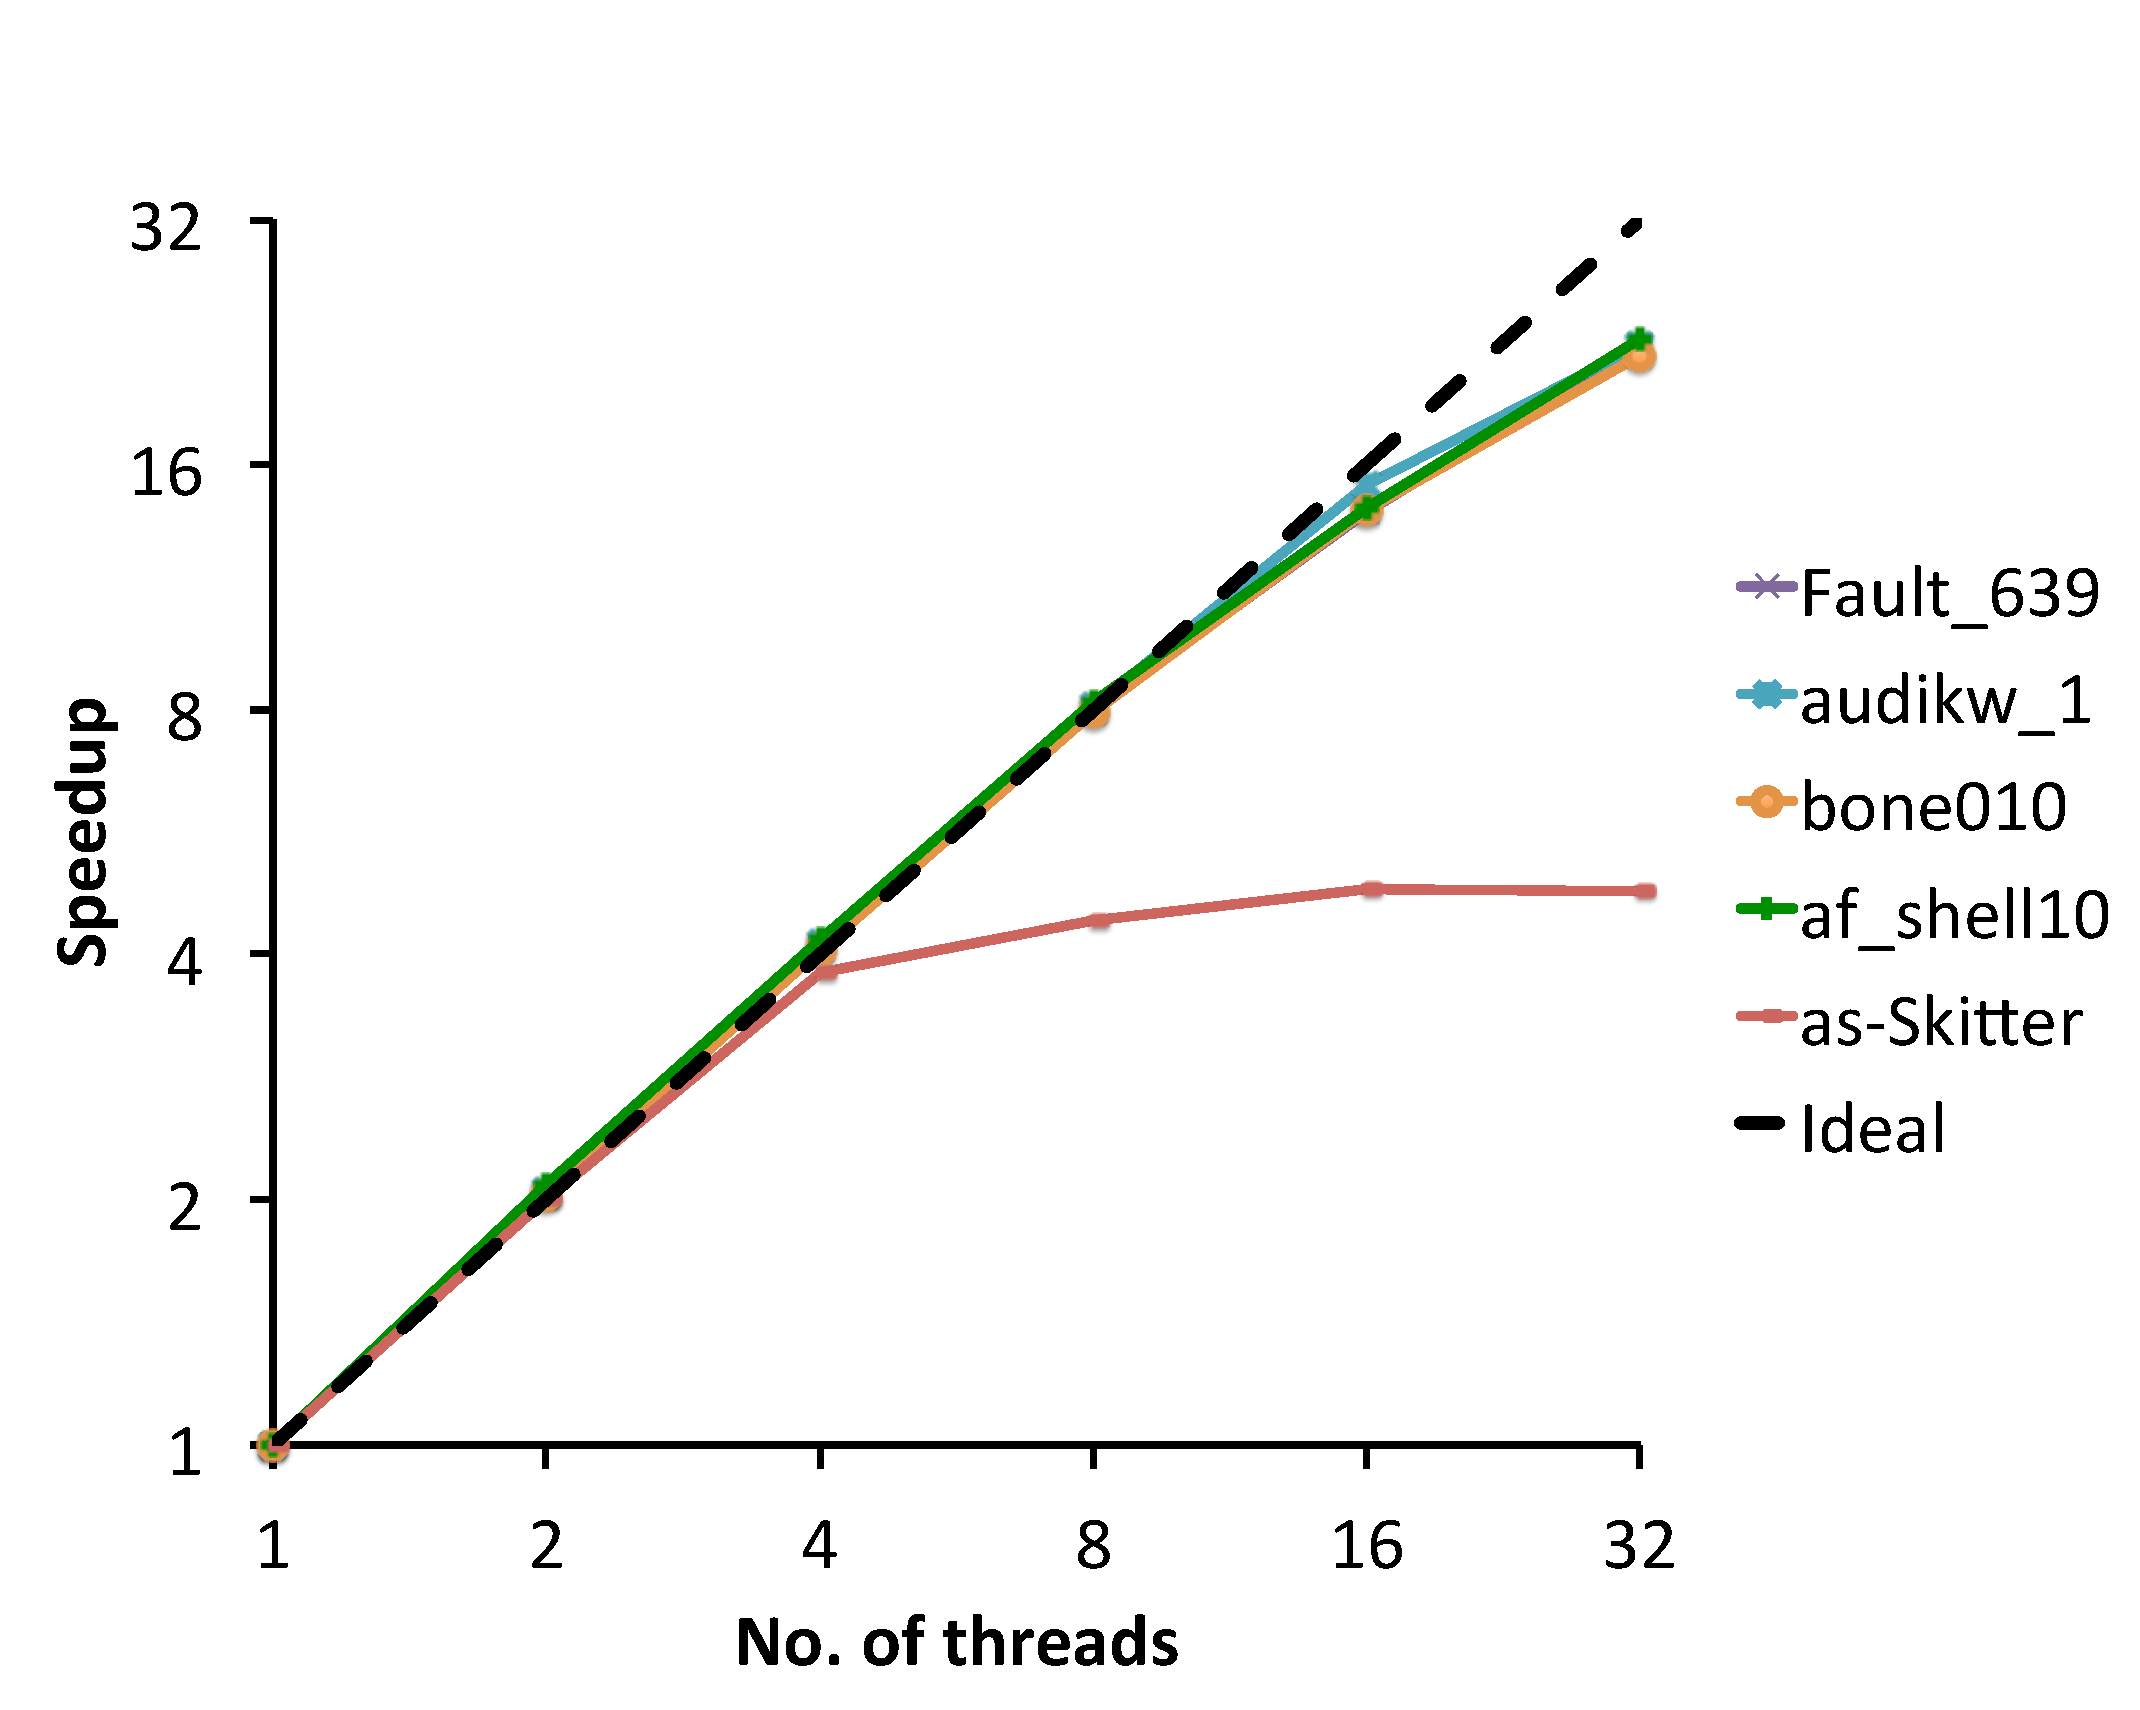
\includegraphics[scale=0.21]{parallel_realworld_speedup.pdf}
    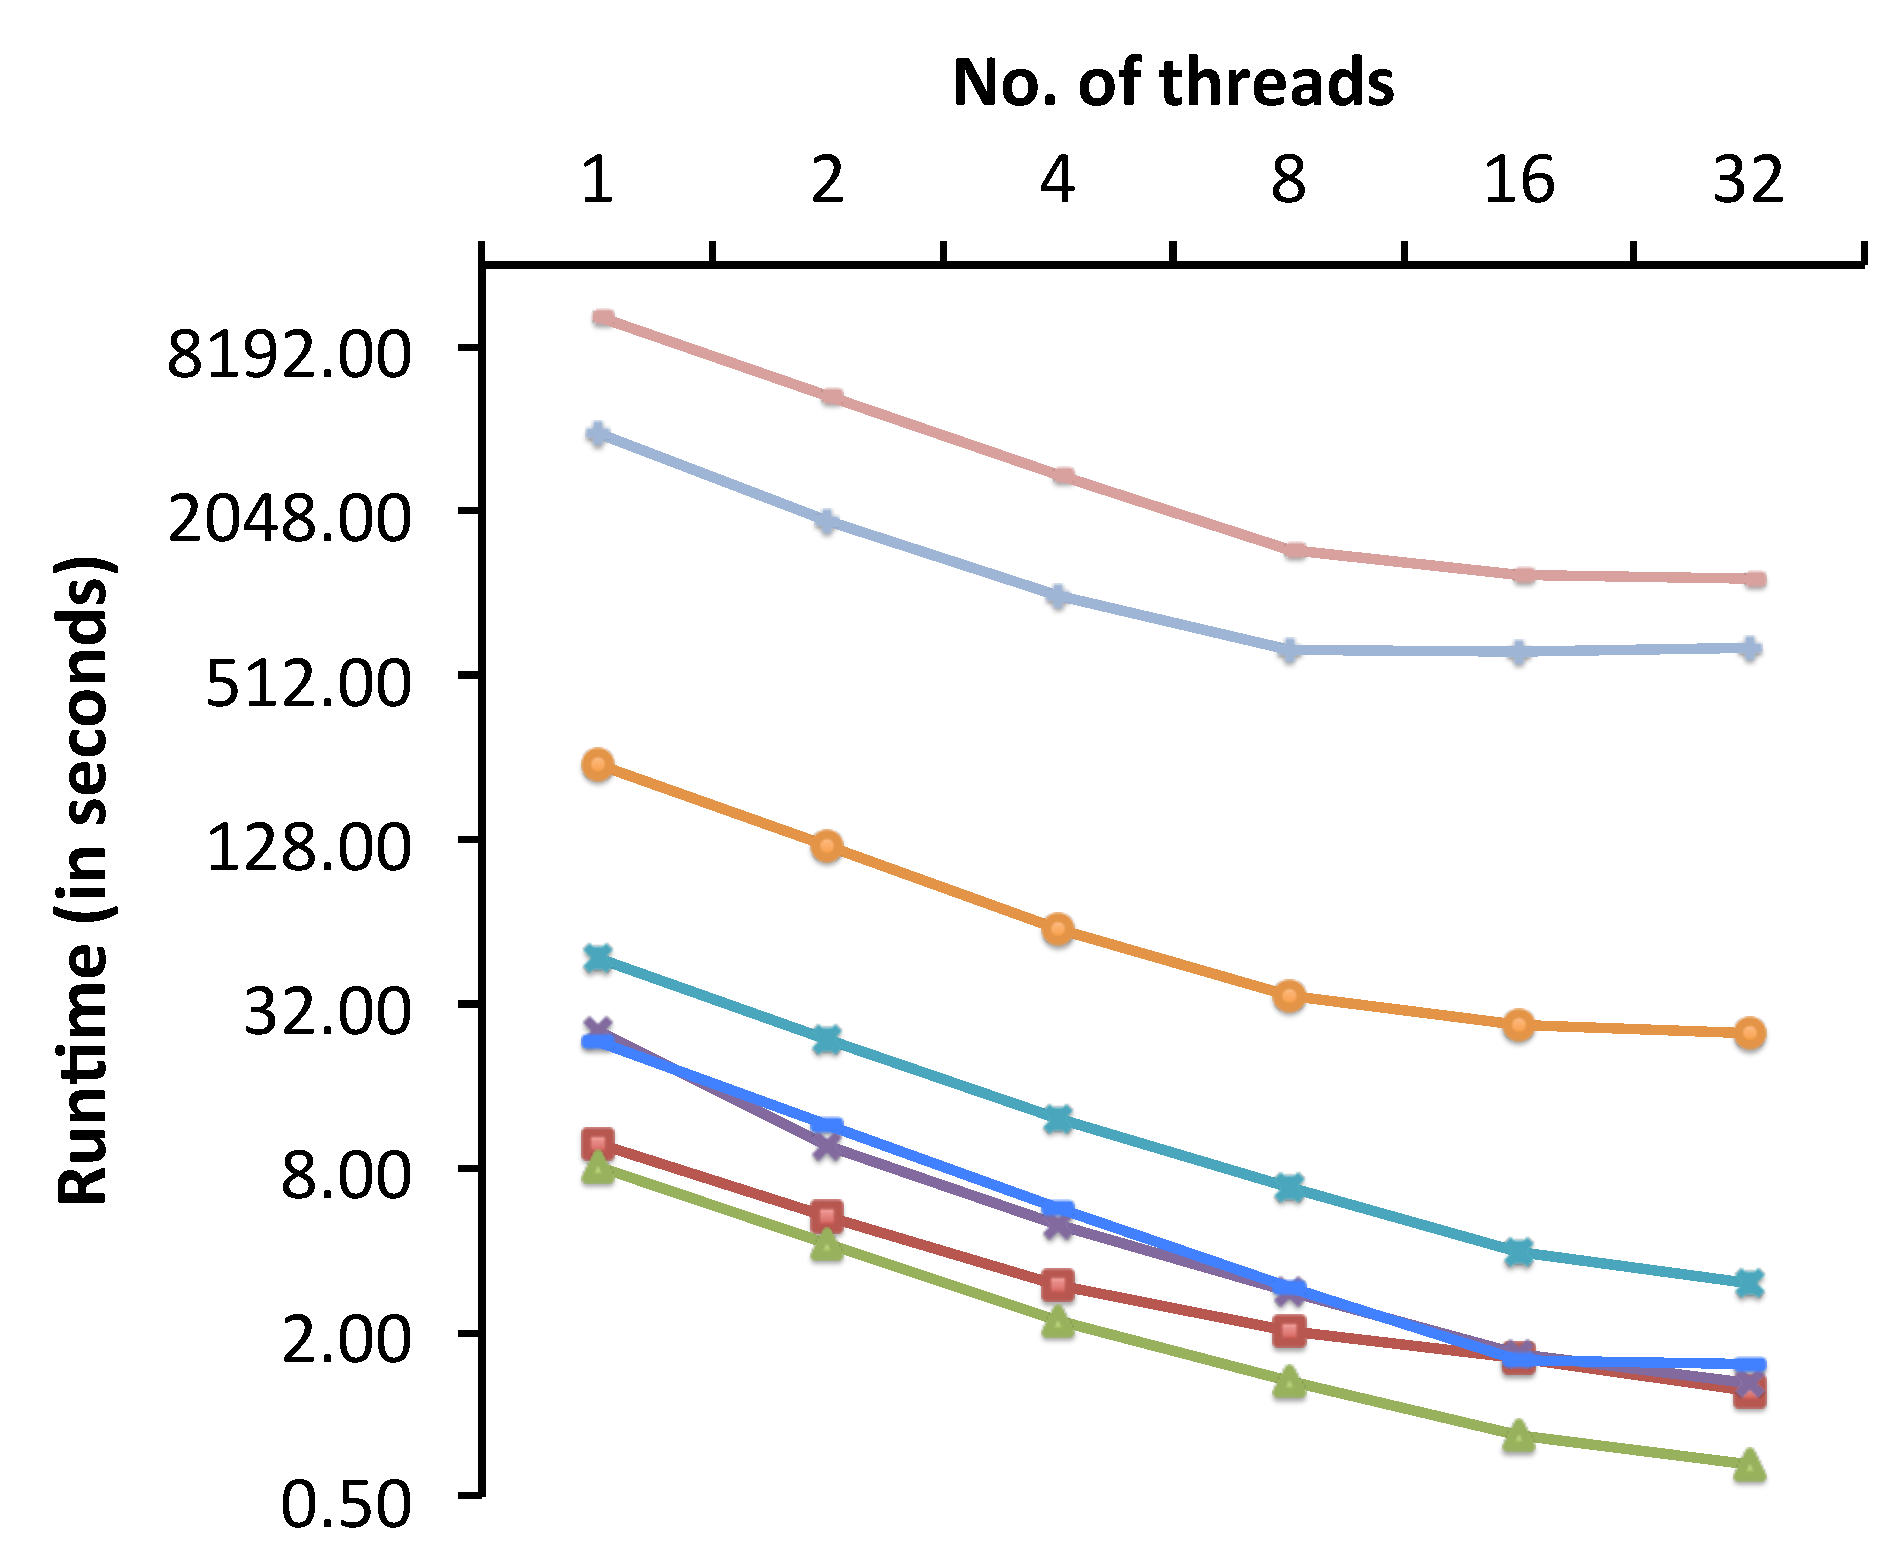
\includegraphics[scale=0.21]{parallel_other_timing.pdf}
    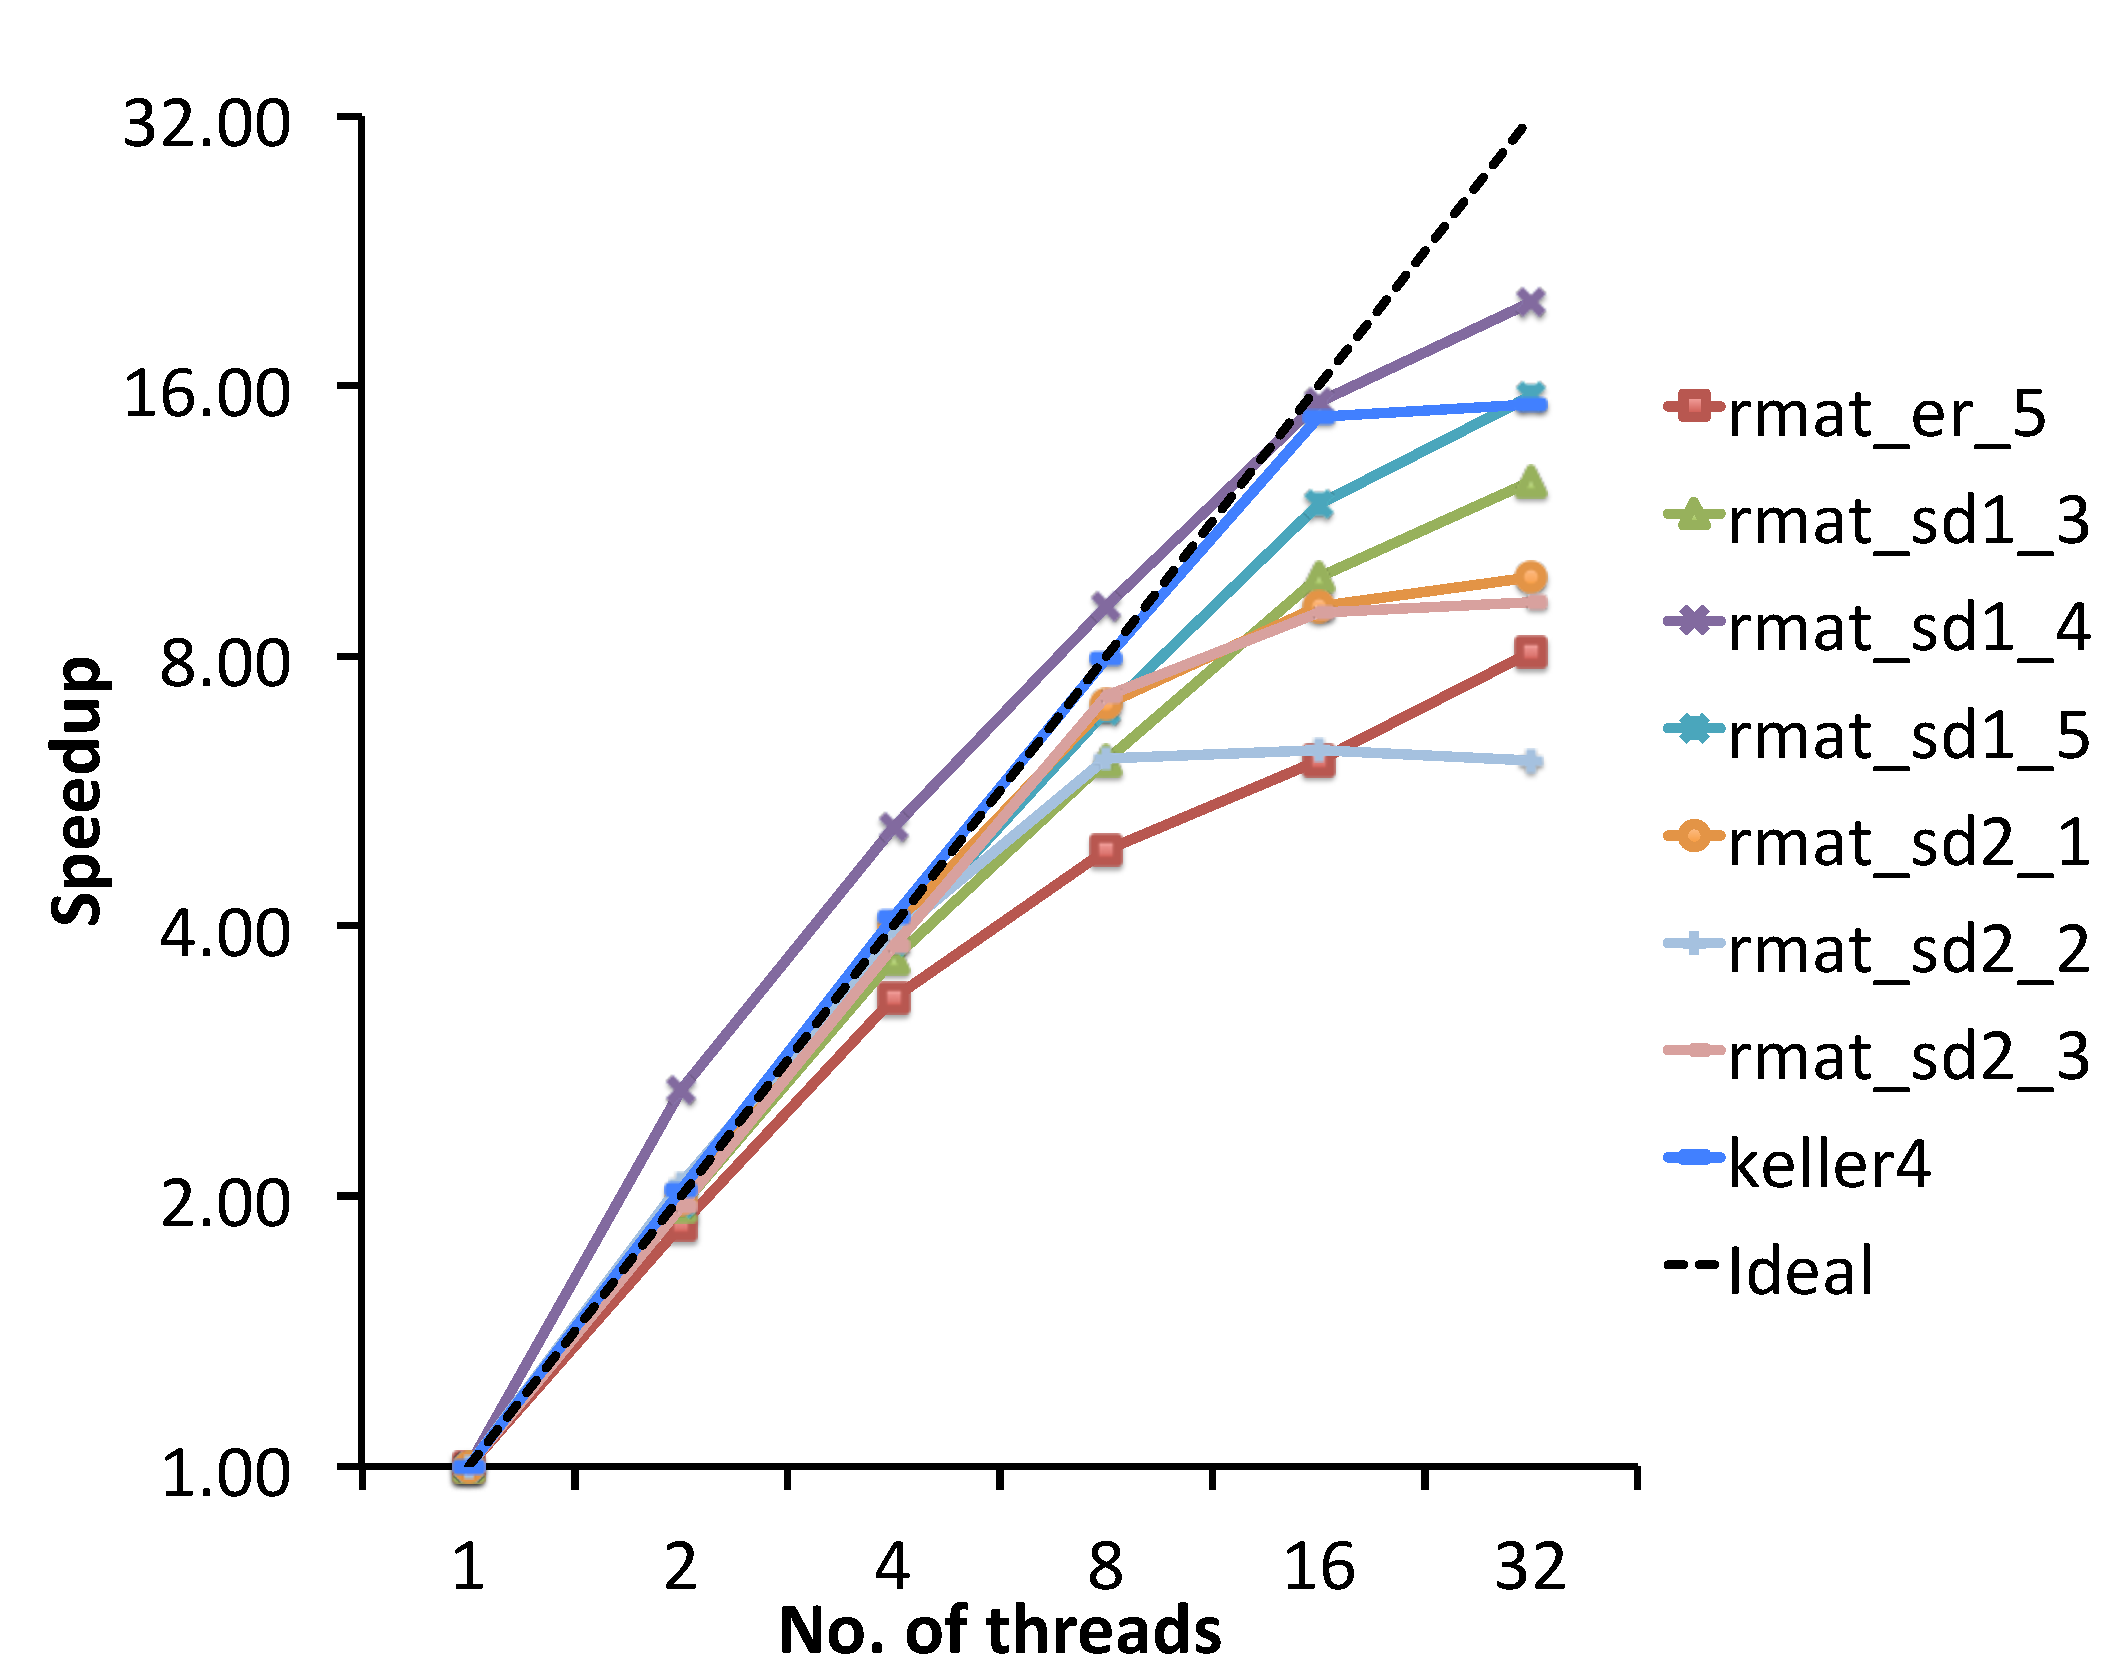
\includegraphics[scale=0.21]{parallel_other_speedup.pdf}
    
%%\vspace{-30pt}
 \caption{Performance (timing and speedup plots) of shared-memory parallelization on graphs in the test-bed. The top set of figures show performance on the real-world graphs, whereas the bottom set show results for the RMAT graphs. Graphs whose sequential runtime is less than 5 seconds were omitted.}
\label{fig-parallel_perf}
\end{figure}


Figure \ref{fig-parallel_perf} shows the timings and speedups we obtained for the real-world and RMAT graphs separately. We omitted graphs whose sequential runtimes were less than 5 seconds as they were too low to measure and do meaningful assessment of parallelization performance. For most of the real-world graphs, one can see from the figure that we obtained near-linear scaling of runtimes and speedups when up to 16 threads are used. The only exception is the graph 
{\emph as-Skitter}. The relatively poorer scaling there is likely due to the fact that the instance has a relatively large maximum clique, and hence the core (thread) which computes it spends relatively large amount of time computing it while other cores (threads) which have completed their processing of the remaining vertices remain idle. 
For the other instances of the real-world graphs, the maximum speedup we obtained 
while using 32 cores/threads is around 22$\times$. 

For the RMAT graphs, it can be seen that the scaling of the runtime and speedups vary with the structures (RMAT parameters) of the instances. We observed super-linear speedups for a couple of the instances, {\bf which
happens as a result of some unfruitful searches in the branch-and-bound procedure being discovered early
as a result of parallel processing. This phenomenon is better exploited and more fully explored in other works in the literature such as  \cite{a6040618}. }
For the other instances, the algorithm scales fairly well up to 8 threads, and begins to
degrade thereafter. The speedups we obtained range between 6$\times$  to 20$\times$ when 32 threads are used.





%The effects of pruning could, although, be tolerably compromised in order to enable the parallel computation by allowing the processors to use the locally computed maximum clique value as the lower bound for pruning until regular synchronization steps, during which it is updated to the global value of the maximum clique across all processors.

%When done in parallel, the for loop in Algorithm \ref{alg:mClq} can be distributed among different $p$ computational units which can compute different values for $max$ in parallel. In the next step, a reduce operation can be used to find the maximum of the $p$ values.

%In this section we show the results of parallelization of our exact algorithm on shared memory architectures. In our algorithm, there is no dependency or strict order in which the vertices have to be computed unlike other previous algorithms. The sizes of the largest cliques containing different vertices can be computed mostly independently, and thus can be done in parallel by different computational units.


%\begin{figure}
%        \centering
%        \begin{subfigure}[b]{0.5\textwidth}
%                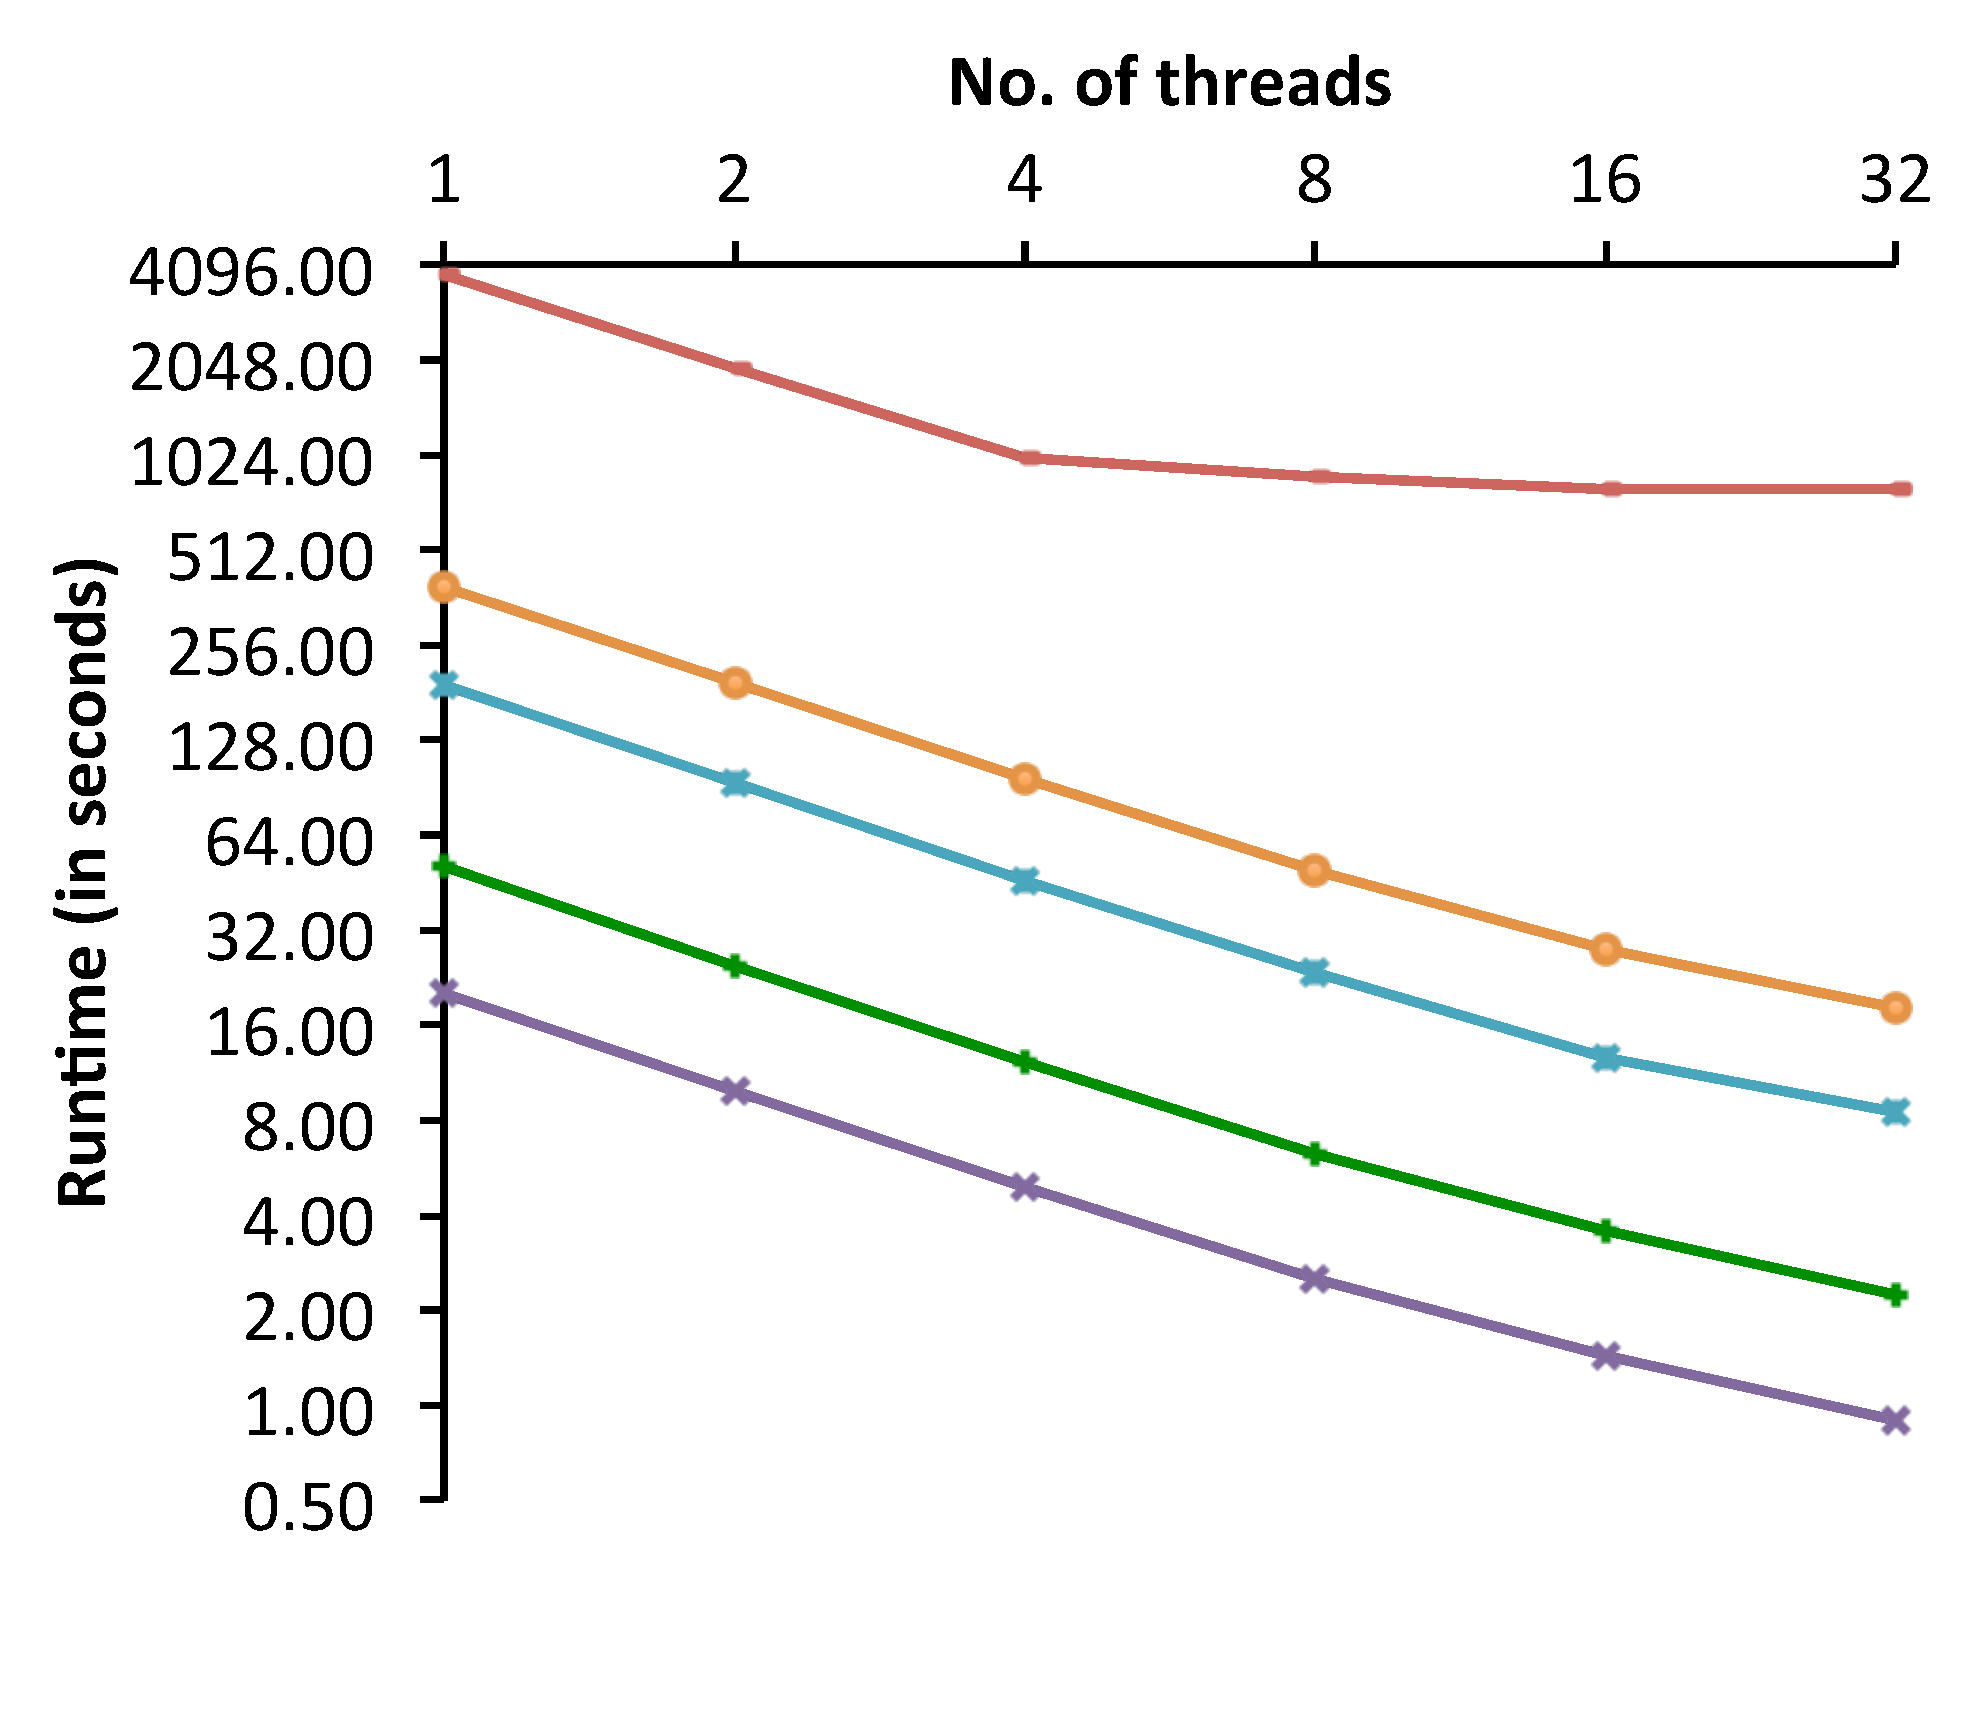
\includegraphics[width=\textwidth]{parallel_realworld_timing.pdf}
%                \caption{Timing results}
%                \label{fig:timing_realworld}
%        \end{subfigure}%
%        ~ %add desired spacing between images, e. g. ~, \quad, \qquad etc.
%          %(or a blank line to force the subfigure onto a new line)
%        \begin{subfigure}[b]{0.5\textwidth}
%                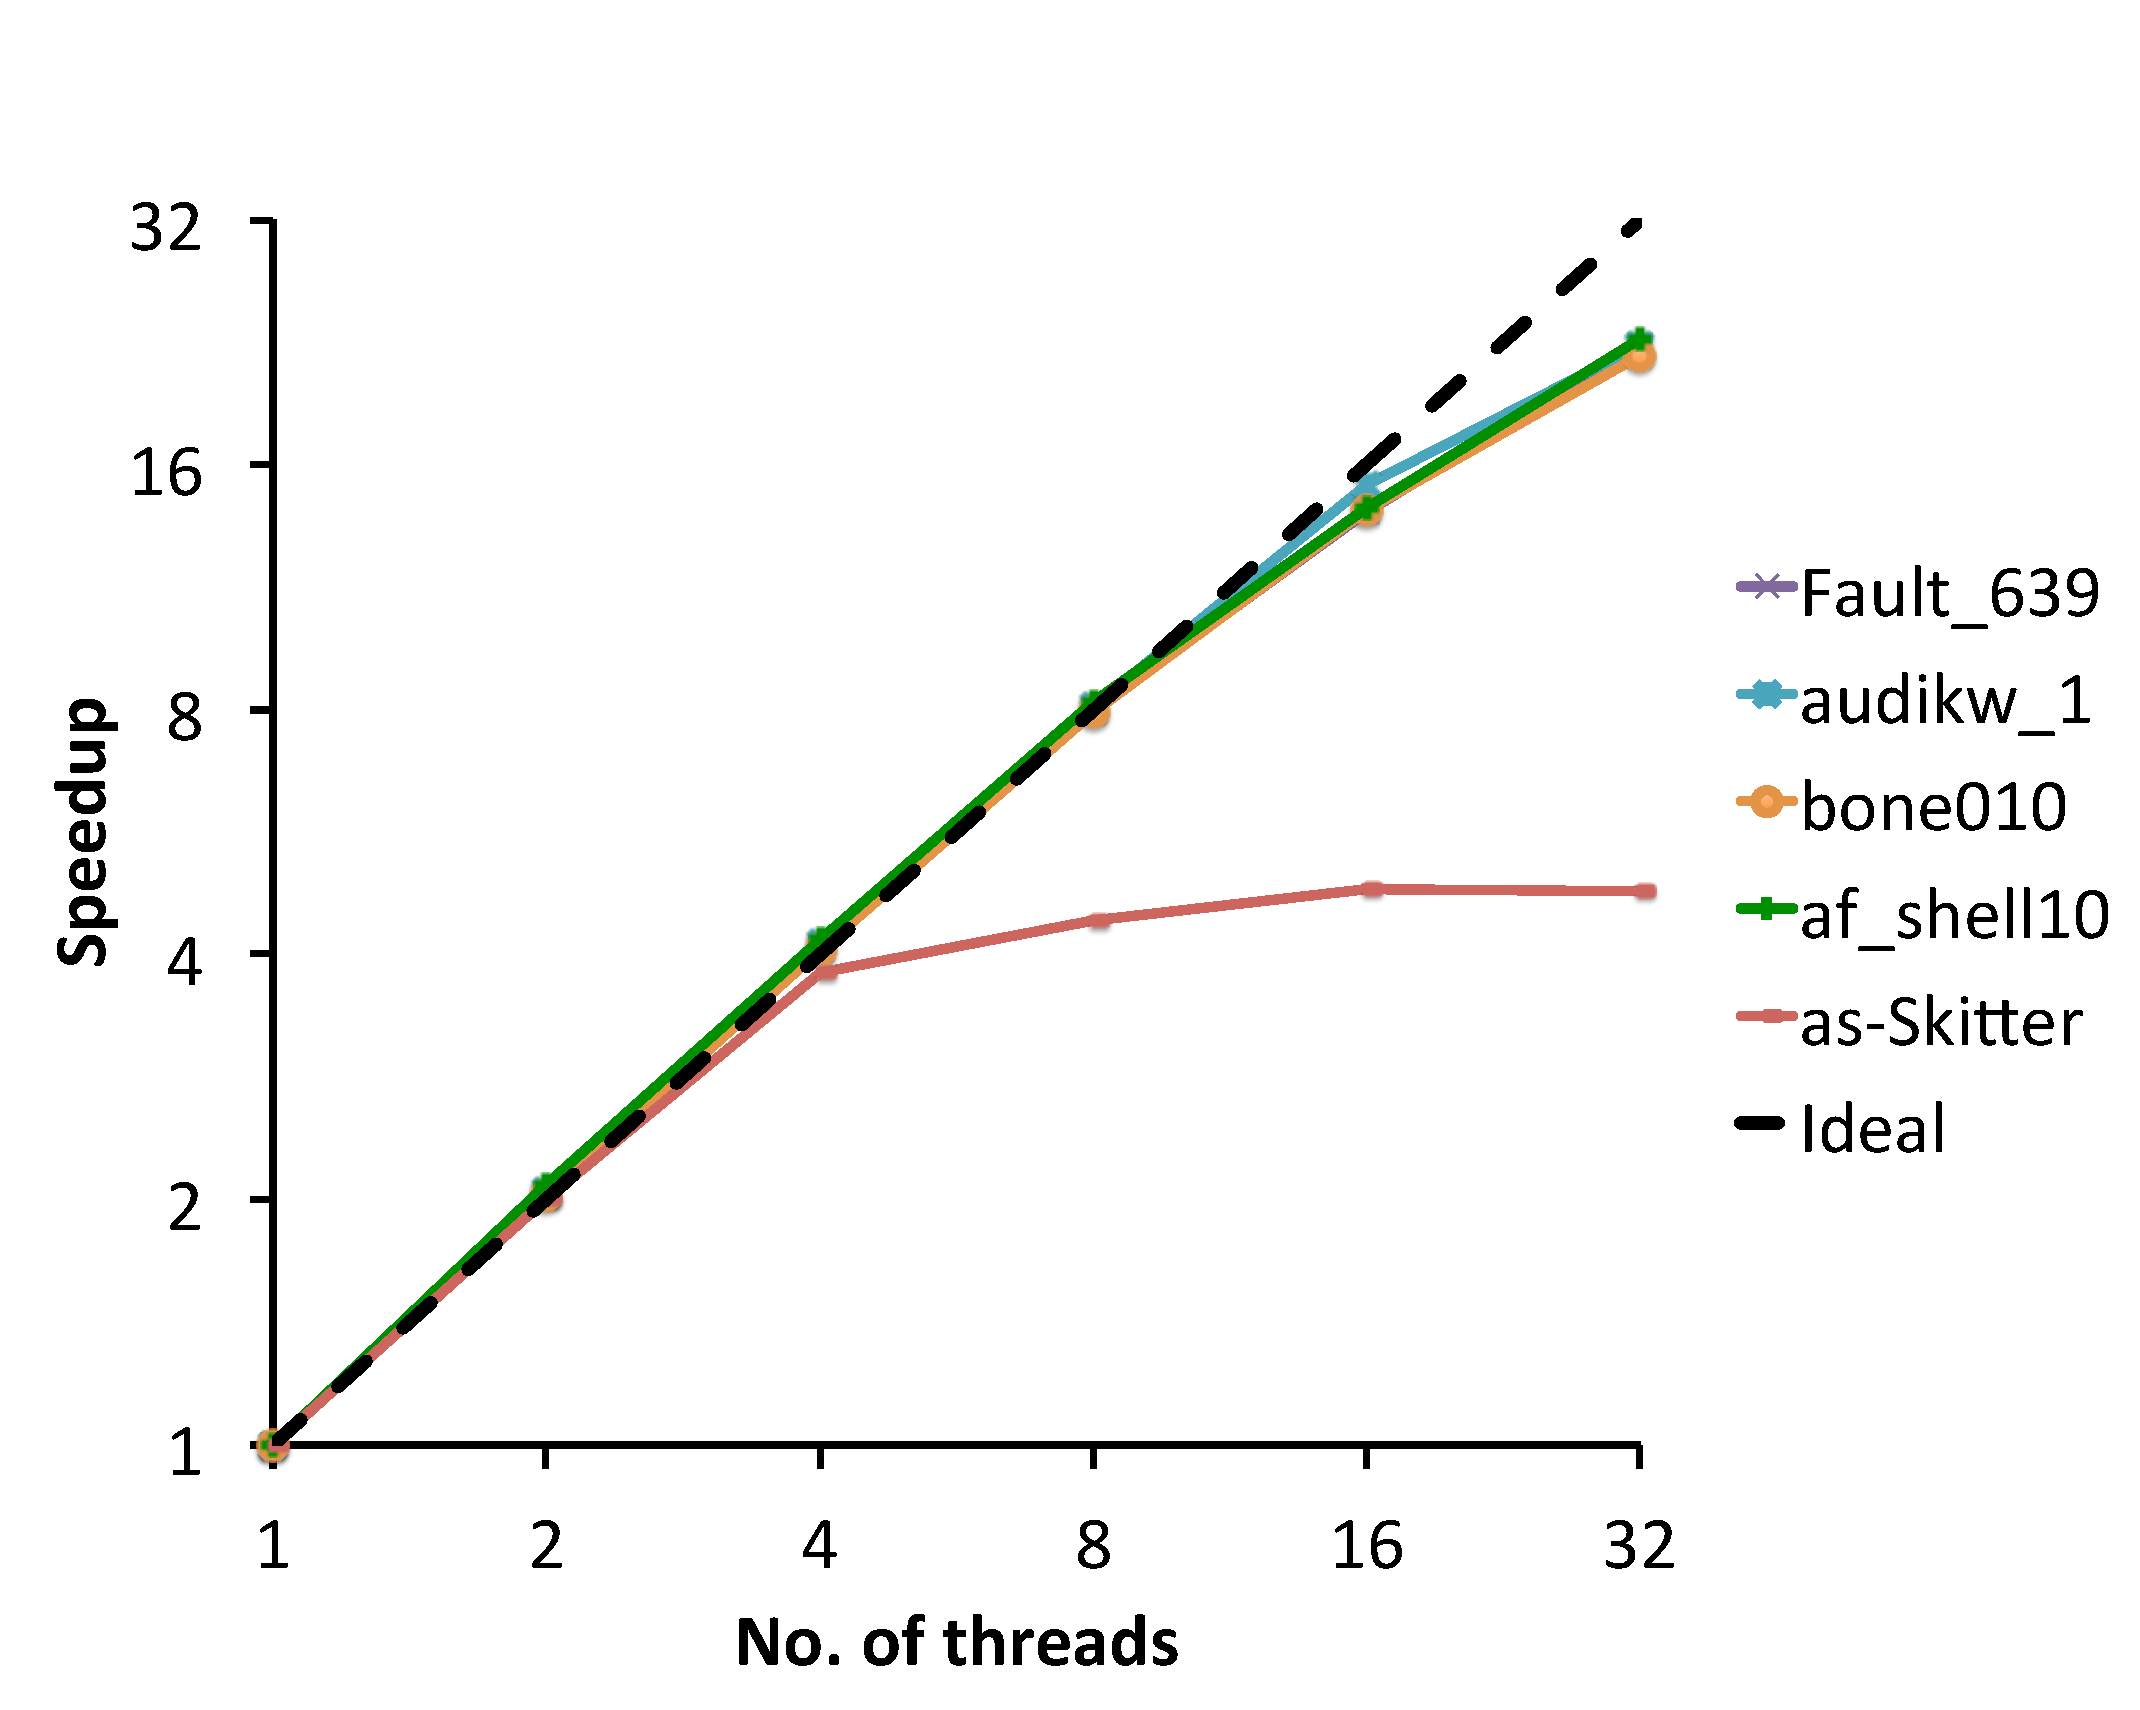
\includegraphics[width=\textwidth]{parallel_realworld_speedup.pdf}
%                \caption{Speedup results}
%                \label{fig:speedup_realworld}
%        \end{subfigure}
%        \caption{Performance of shared-memory parallelization on real-world graphs}\label{fig:animals}
%\end{figure}
%
%
%\begin{figure}
%        \centering
%        \begin{subfigure}[b]{0.5\textwidth}
%                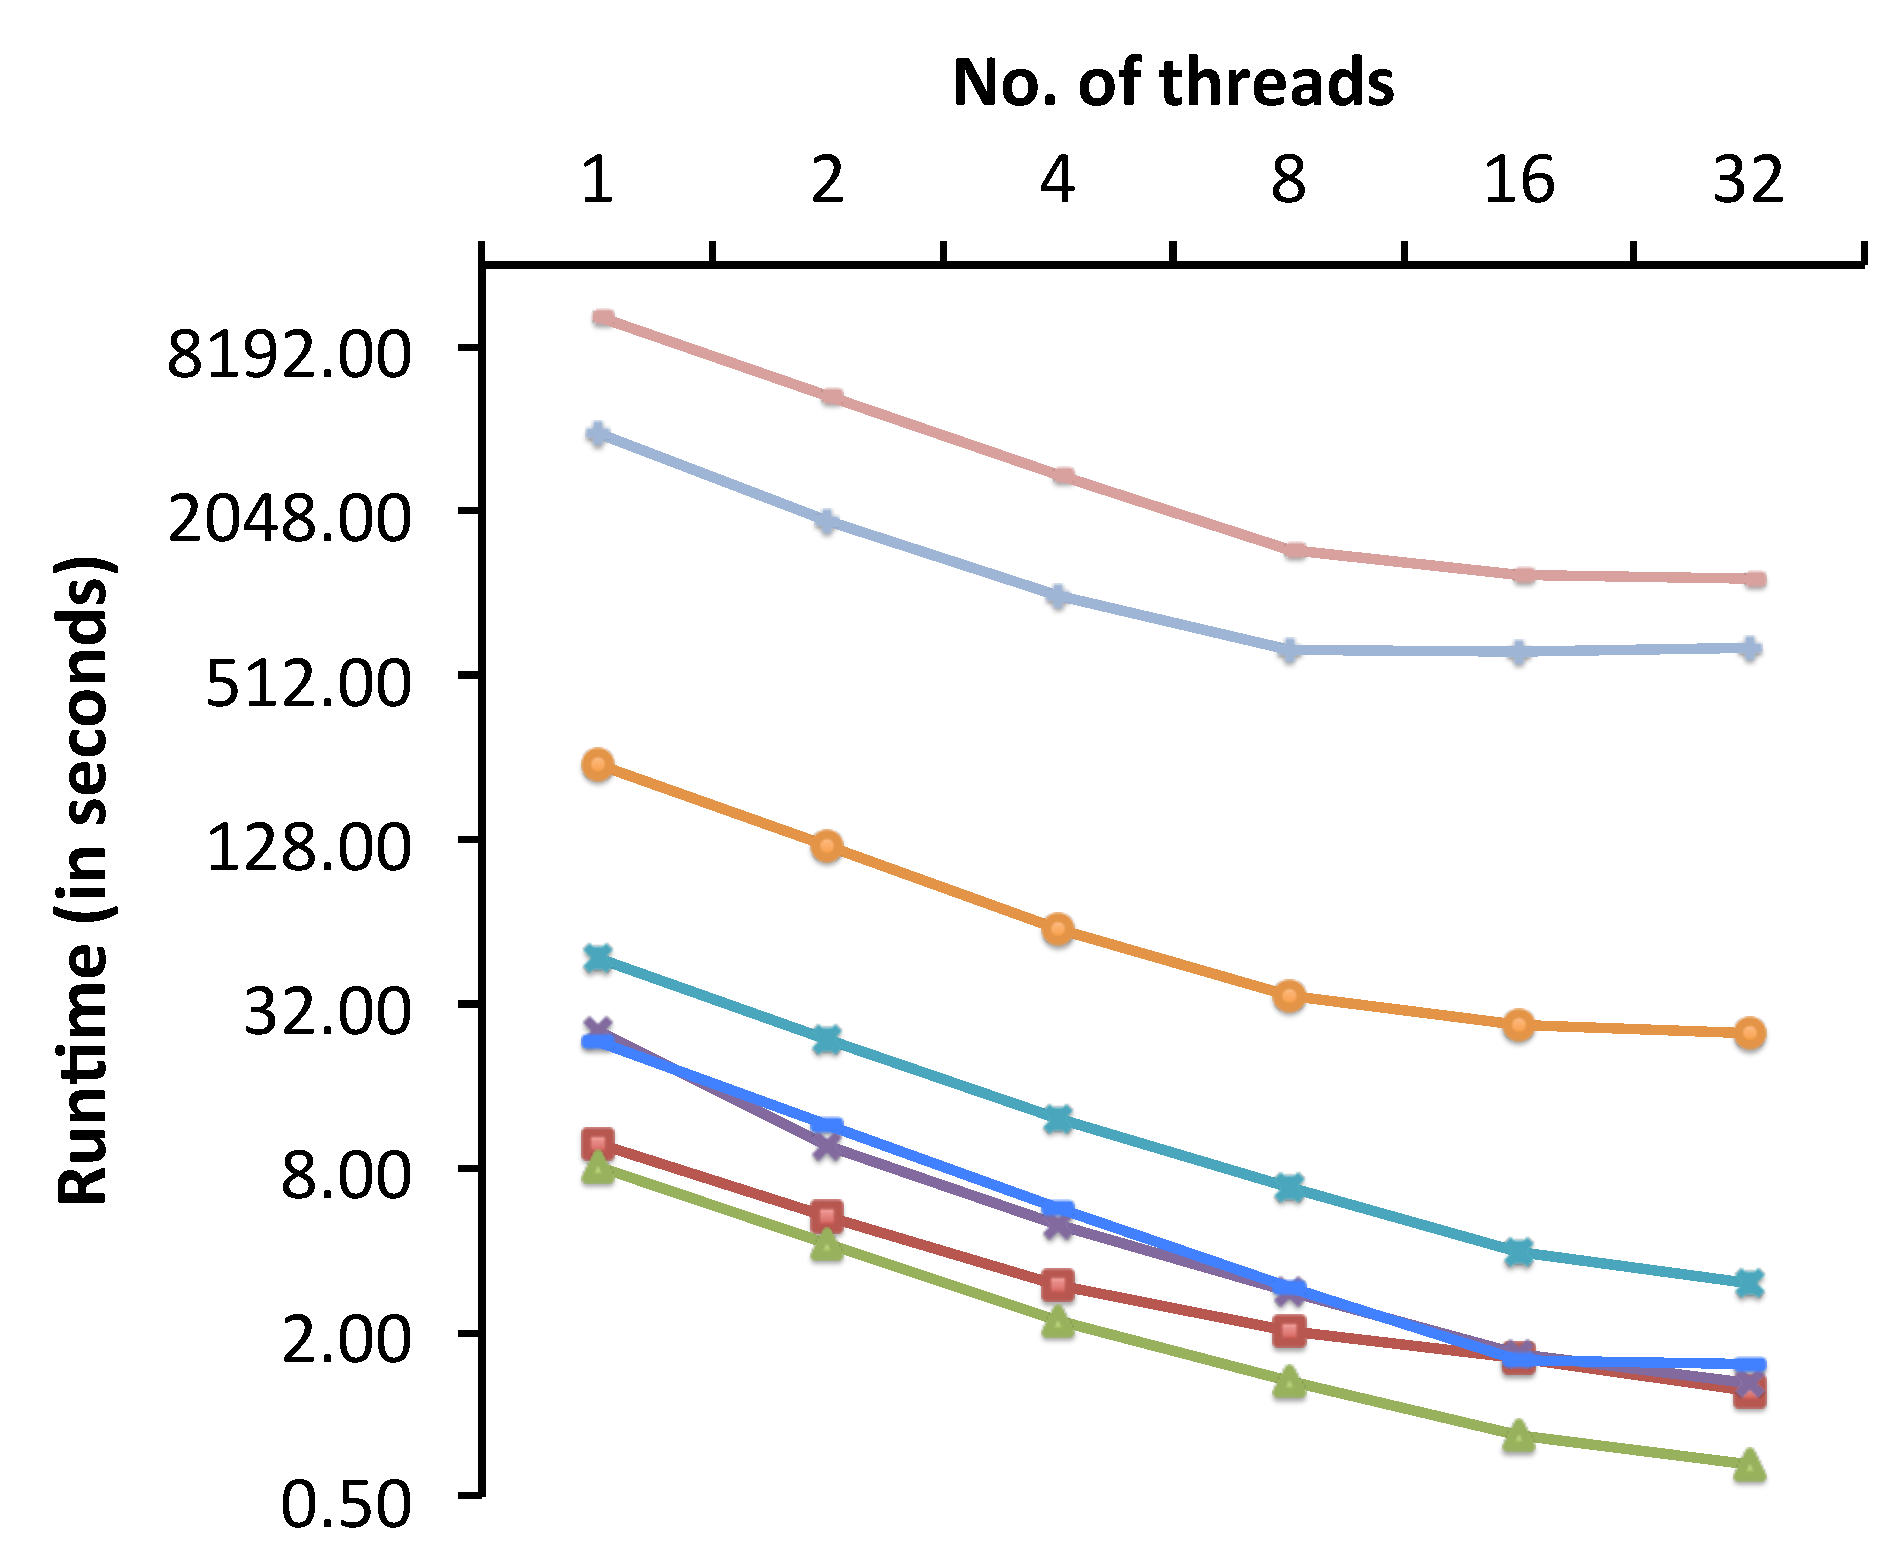
\includegraphics[width=\textwidth]{parallel_other_timing.pdf}
%                \caption{Timing results}
%                \label{fig:timing_realworld}
%        \end{subfigure}%
%        ~ %add desired spacing between images, e. g. ~, \quad, \qquad etc.
%          %(or a blank line to force the subfigure onto a new line)
%        \begin{subfigure}[b]{0.5\textwidth}
%                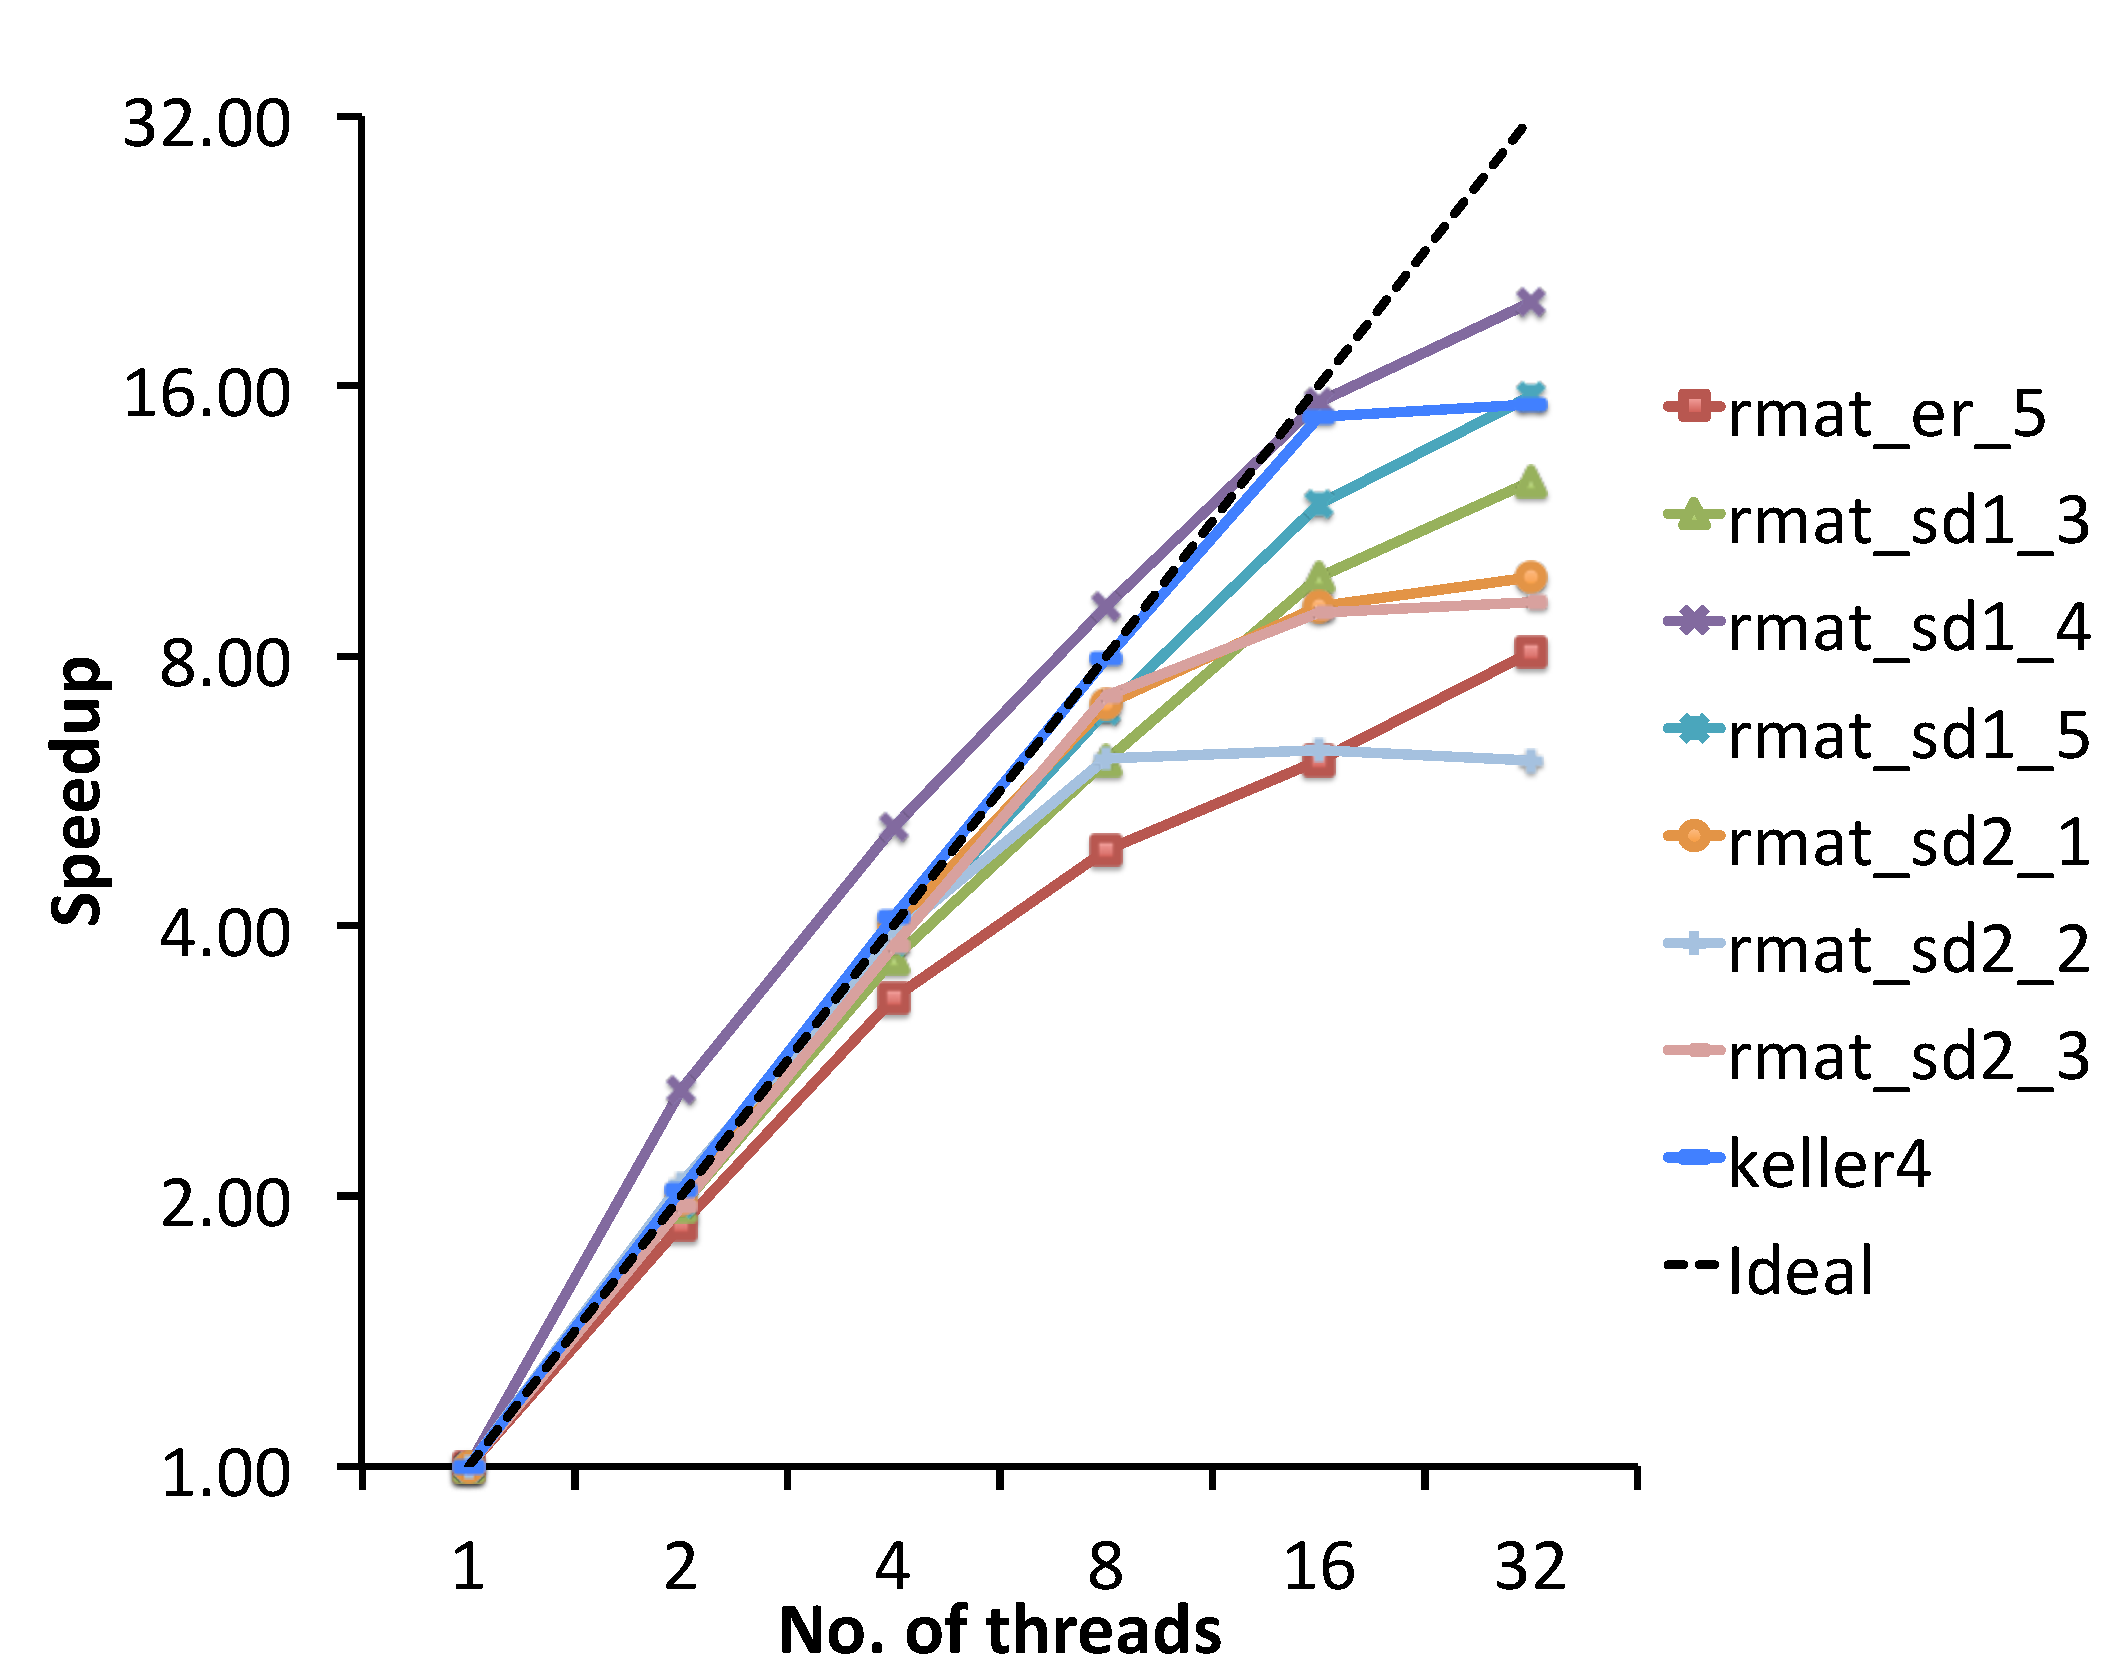
\includegraphics[width=\textwidth]{parallel_other_speedup.pdf}
%                \caption{Speedup results}
%                \label{fig:speedup_realworld}
%        \end{subfigure}
%        \caption{Performance of shared-memory parallelization on real-world graphs}\label{fig:parallel_perf}
%\end{figure}
%





